\chapter{Architectural design}

\section{Overview}
The system-to-be that will be implemented for PowerEnJoy is made of three main layers: client, application server and database.

\begin{figure}[h]
	\centering
	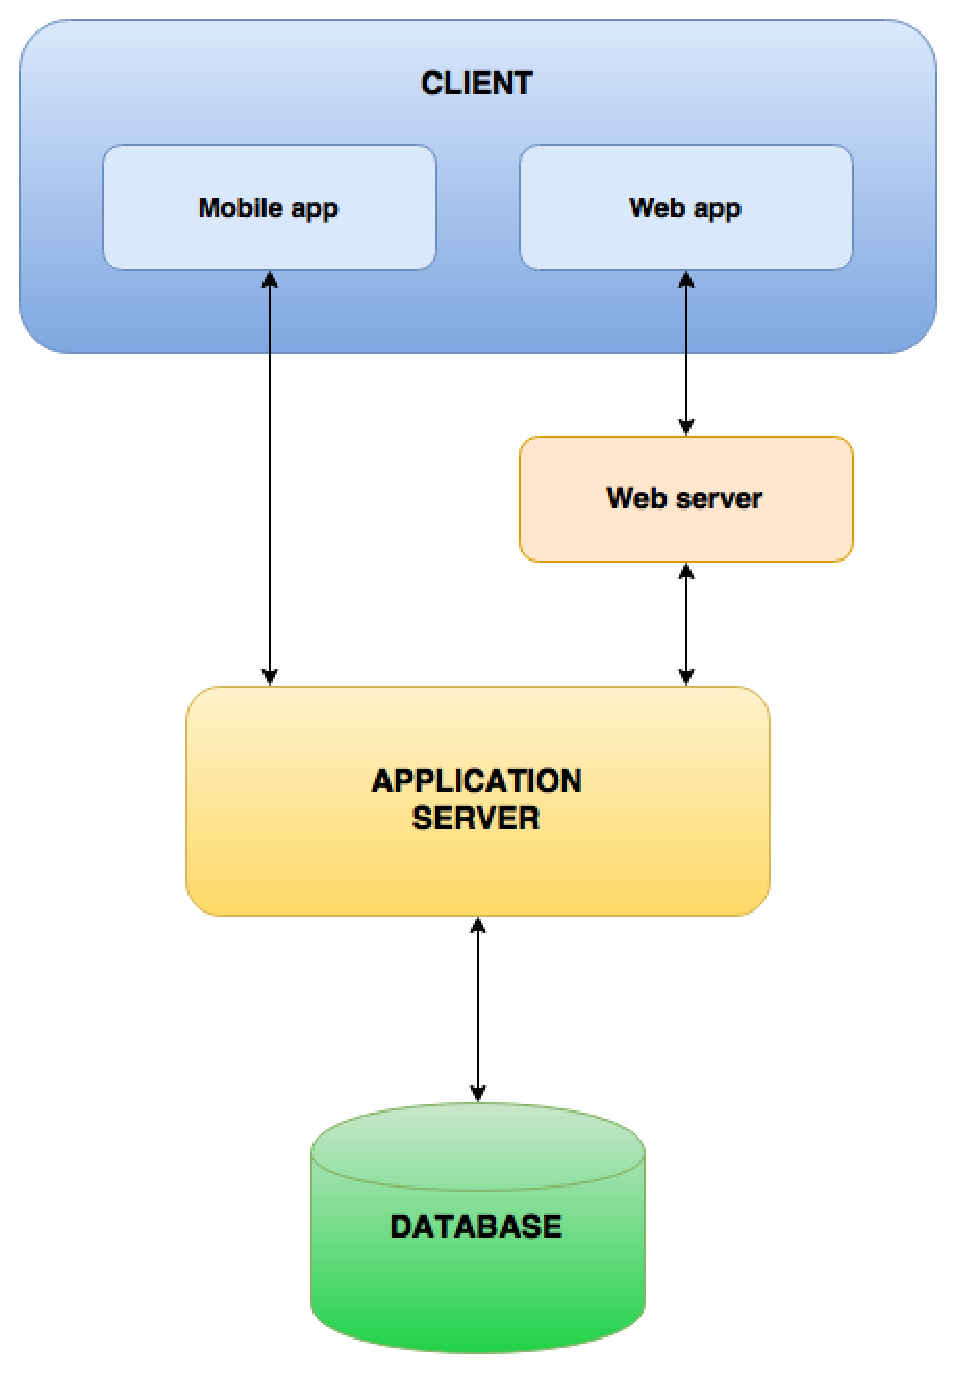
\includegraphics[width=7cm,keepaspectratio]{figures/layers.eps}
	\caption{Layers of the system}
	\label{fig:layers}
\end{figure}

\begin{itemize}
	\item \emph{Client}. It is the presentation layer and provides two different interfaces, a mobile app and desktop version to be used via web. \\ The former is intended for phone and tablets and straightly interacts with the application server layer. \\ The latter is a web app, intended then for browsers, which interacts with the web server, a middleware in charge of providing the model of the layout and handling the events coming from the web app.
	
	\item \emph{Application server}. It is the logic layer of the system. It includes all the business logic and provides web services so that users can interact with this layer from both the interfaces.
	
	\item \emph{Database}. It is the data layer of PowerEnJoy. It interacts only with the application server, receiving from it requests to retrieve, update, create or delete the data stored. It provides the interfaces that allow the application layer to execute these operations. 
\end{itemize}

\newpage
\section{Component view}
\begin{figure}[h]
	\centering
	\includegraphics[height=15.2cm,keepaspectratio]{figures/component_view.eps}
	\caption{Component view of PowerEnJoy}
	\label{fig:component_view}
\end{figure}

\newpage
\section{Deployment view}
\begin{figure}[h]
	\centering
	\includegraphics[width=\linewidth,keepaspectratio]{figures/deployment_view.eps}
	\caption{Deployment view diagram of the system}
	\label{fig:deployment_view}
\end{figure}

\section{Runtime view}
This section describes the system components involved and the related interactions for some of the use cases reported in the RASD.

The map manager is an interface that acts as a router to communicate between the Client/User and with the system. In the run time view sequence diagram,
the map manager is not shown mostly in all the diagrams. But in the individual explanation of the sequence diagram, its functionality is explained.

Each and every component are separated for specific functionality. This is done in order to achieve better performance and re-usability of the code.

\subsubsection{Selection of available car}
\begin{figure}[t]
	\centering
	\includegraphics[width=\linewidth,keepaspectratio]{figures/selection_available_car_runtime.eps}
	\caption{Sequence diagram for the selection of the available car}
	\label{fig:selection_available_car_runtime}
\end{figure}

The Client/User wants to select an available car. Only after successful login, the Client/User will be able to select the car. A Login manager takes care of this credential verification.
After successful verification of the user credentials, the Client/User can send a request to select an available Car through the map manager which transfers the request to the selection
manager. This indeed interacts with the selection controller to display the list of available cars.

The controller interacts with another component called availability helper.
This availability helper communicates with all the cars and checks which cars are available. This check happens in a loop continuously After finding the list of available cars, then the response is transferred selection controller and finally it is transferred to the Client/User. After this, the user/client can select only one available car for the reservation.

\subsubsection{Reservation of selected car}
\begin{figure}[t]
	\centering
	\includegraphics[width=\linewidth,keepaspectratio]{figures/reservation_runtime.eps}
	\caption{Sequence diagram for the reservation of the selected car}
	\label{fig:reservation_runtime}
\end{figure}

The reservation confirmation of a car can happen only after selection of the available car. So the sequence of the user's request for the reservation starts from the selection manager. It transfers the request to the reservation manager for the confirmation. The reservation controller is a component that sends another request to the availability helper
to change the tag of the car selected.

The availability helper interacts with the car and changes the tag as ``reserved''. The availability helper starts a counter timer immediately after changing the tag by setting a time for 60 minutes. This tag will hold reserved only for upto 60 minutes. Now, the response is sent back to the reservation controller which is finally sent to the Client/User as a confirmed reservation.

\subsubsection{Selection of special parking areas}
\begin{figure}[t]
	\centering
	\includegraphics[width=\linewidth,keepaspectratio]{figures/special_parking_area_runtime.eps}
	\caption{Sequence diagram for the selection of special parking areas}
	\label{fig:special_parking_area_runtime}
\end{figure}

The Client/User requests for a special parking area to get a discount. So, he/she selects the option during the ride to the system through the map manager. The map manager
acts as an interface and transfers the request to the ride manager. The ride manager provides an interface to communicate with the ride controller during the ride. 

This component asks to display the available list of special parking areas nearby. So, the parking manager accepts this request while the parking controller checks the availability of special parking areas and sends the list of available special parking areas to the Parking manager. The parking controller does a check continuously in a loop. If there are no special parking areas available, then it sends an response with result as zero and suggests list of safe parking areas to the parking manager. This requests are finally sent as a response to the user/client.

\subsubsection{Enable money saving option for discount}
\begin{figure}[t]
	\centering
	\includegraphics[width=\linewidth,keepaspectratio]{figures/money_saving_option_runtime.eps}
	\caption{Sequence diagram for the activation of the money saving option}
	\label{fig:money_saving_option_runtime}
\end{figure}

The Client/User wants to select/enable money saving option for availing a discount. In order to do that, he/she must select the final destination through the map manager. The map manager asks to select the final destination immediately after selecting the money saving option. After entering the final destination, the request is transferred to the Parking controller through the parking manager to select the parking areas that have a discount.

To check to discount applicability, the parking controller communicates with the discount and penalty manager. The discount controller checks if the parking area is applicable for a discount and calculates the discount. This discount information along with the parking area is sent as a response to the Client/User through the map manager.

\section{Selected architectural styles and patterns}
As described before, our application will be divided into three main layers:
\begin{itemize}
	\item Database (for the storing of permanent data)
	\item Application Server (for the business logic)
	\item Client (for the interaction between user and system)
\end{itemize}

RESTful API with JSON used by clients (both mobile apps and web browsers) to interact with the application layer. Users have to authenticate through specific API calls via HTTP basic authentication for each request.

As regards the patterns for designing PowerEnJoy, the Model-View-Controller one has been widely taken into account. MVC is a software design pattern for implementing user interfaces on computers. It divides a given software application into three interconnected parts, so as to separate internal representations of information from the ways this is presented to the user.